% =========================
% WCCI 2026 Full Paper
% Edge-Cell Graph Encoding and Fixed-Point Arithmetic for FPGA Growing Neural Gas
% =========================
\documentclass[conference]{IEEEtran}

% IEEE-style citations (BibTeX)
\usepackage{cite}

\usepackage{amsmath,amssymb,amsfonts}
\usepackage{graphicx}
\usepackage{algorithm}
\usepackage{algorithmic}
\usepackage{multirow}
\usepackage{array}
\usepackage{url}
\usepackage{booktabs}
\usepackage{listings}
\usepackage{xcolor}
\usepackage{enumerate}

% Code listing configuration
\lstset{
  basicstyle=\ttfamily\footnotesize,
  keywordstyle=\color{blue},
  commentstyle=\color{gray},
  stringstyle=\color{red},
  breaklines=true,
  frame=single,
  captionpos=b,
  language=VHDL
}

\begin{document}

\title{Edge-Cell Graph Encoding and Fixed-Point Arithmetic for FPGA Growing Neural Gas}
\author{
\IEEEauthorblockN{Teuku Zikri Fatahillah\IEEEauthorrefmark{1}, Raditya Artha Rochmanto\IEEEauthorrefmark{1}\IEEEauthorrefmark{2}, Achmad Fahrul Aji\IEEEauthorrefmark{1}\IEEEauthorrefmark{2},\\
Anhar Risnumawan\IEEEauthorrefmark{1}\IEEEauthorrefmark{3}, Chyan Zheng Siow\IEEEauthorrefmark{1}\IEEEauthorrefmark{4}, Naoyuki Kubota\IEEEauthorrefmark{1}}
\IEEEauthorblockA{\IEEEauthorrefmark{1}Department of Mechanical Systems Engineering, Graduate School of Systems Design\\
Tokyo Metropolitan University, 6-6 Asahigaoka, Hino, Tokyo 191-0065, Japan\\
\{teuku-fatahillah, rochmanto-artha, achmad-aji, risnumawan-anhar\}@ed.tmu.ac.jp, \{siow-zheng, kubota\}@tmu.ac.jp}
\IEEEauthorblockA{\IEEEauthorrefmark{2}Department of Electrical Engineering, Politeknik Negeri Semarang, Indonesia}
\IEEEauthorblockA{\IEEEauthorrefmark{3}Mechatronics Engineering Division, Politeknik Elektronika Negeri Surabaya, Indonesia}
\IEEEauthorblockA{\IEEEauthorrefmark{4}Changsha Cultural and Creative Arts Vocational College, China}
}

% BibTeX style control (prevents dashed repeated author names like "------")
\bstctlcite{IEEEexample:BSTcontrol}
\maketitle

\begin{abstract}
We present an FPGA implementation of Growing Neural Gas (GNG) on a Sipeed Tang Nano~9K (Gowin GW1NR-9C) as a bounded-memory hardware substrate for online self-organizing clustering. The design uses an FSM datapath with BRAM-based storage, integer fixed-point arithmetic (Q8/Q16), and a compact \emph{edge-cell graph encoding} that stores the upper-triangular adjacency as 8-bit age+1 values, avoiding dense adjacency matrices and dynamic memory allocation. The complete design is implemented without any soft-core processor or floating-point unit, and is evaluated on Two Moons and Concentric Circles benchmarks. The platform establishes a hardware foundation for deploying continual self-organizing clustering on resource-constrained edge devices.
\end{abstract}

\begin{IEEEkeywords}
Growing Neural Gas, self-organizing clustering, FPGA, integer fixed-point arithmetic, unsupervised learning, topology learning, edge computing
\end{IEEEkeywords}


% ============================================================
\section{Introduction}
Intelligent systems deployed on small aerial robots, micro-UAV swarms, and field robots increasingly demand on-board unsupervised adaptation for tasks such as online topology formation, novelty detection, and structure discovery. In these dynamic environments, streaming raw sensory data to a cloud backend is often impractical due to intermittent connectivity and latency, so learning must execute locally with bounded per-sample time and predictable state size. Self-organizing clustering algorithms are well suited to this setting because they can discover data structure incrementally without predefined class labels or offline retraining.

Growing Neural Gas (GNG) is a well-established self-organizing clustering algorithm for topology learning and vector quantization~\cite{fritzke1994growing}. Building on earlier self-organizing methods~\cite{kohonen1982self, Kohonen1995SOM} and the growing cell structures framework~\cite{Fritzke1994GCS}, GNG incrementally adapts its graph structure to approximate the input data distribution without retraining cycles. Its sample-by-sample update rule, dynamic node insertion, and edge-aging mechanism make it inherently compatible with incremental learning, where the algorithm continuously refines its representation as new data arrives.

However, deploying GNG at the edge introduces practical challenges: typical embedded targets provide only a few kilobytes of on-chip RAM, lack floating-point hardware, and require deterministic execution timing.

FPGA targets address many of these constraints: they offer custom integer datapaths, synchronous block RAMs (BRAMs) with one-cycle access, and DSP multipliers that execute fixed-width multiplications in a single clock cycle. However, conventional GNG engineering choices remain misaligned with typical small-FPGA constraints. Dense adjacency matrices are particularly mismatched because connectivity storage scales as $O(N^2)$, so even modest caps (e.g., $N_{\max}=40$) make adjacency dominate the memory footprint: a full $40\times 40$ matrix of 8-bit edge ages requires 1,600~B. Floating-point arithmetic incurs either dedicated FPU blocks or slower iterative units, whereas integer-only datapaths map cleanly to FPGA LUTs and DSP slices.

To address these constraints, we propose an FPGA GNG design that combines compressed \emph{edge-cell} graph storage with 16-bit integer arithmetic and shift-based learning-rate approximations, implemented entirely in synthesizable VHDL as a single-clock FSM on the Sipeed Tang Nano 9K. The design stores node state (coordinates, degree, error) in one BRAM and edge state in a second BRAM, and processes each input sample through a sequential pipeline of read-modify-write operations. Under fixed-capacity allocation ($N_{\max}=40$), the proposed edge-cell representation reduces the allocated edge-storage from 1,600~B (dense 8-bit $N_{\max}\!\times\!N_{\max}$ adjacency) to 780~B (upper-triangular half-adjacency), a 51.25\% reduction, while the full GNG state occupies only 1,180~B of BRAM. The main contributions are as follows:
\begin{enumerate}[(i)]
  \item a synthesized FPGA GNG design targeting the Gowin GW1NR-9C FPGA, with integer-only arithmetic and BRAM-mapped node/edge storage;
  \item an \emph{edge-cell} connectivity encoding storing the upper-triangular adjacency as 8-bit \emph{age+1} values (0 = no edge) to minimize BRAM usage and branch complexity;
  \item shift-based Q8/Q16 approximations for winner and neighbor learning rates, enabling single-cycle DSP multiplications without a floating-point unit;
  \item a winner-indexed \emph{fused update pass} that performs error accumulation, error decay, edge aging, neighbor movement, and over-age edge pruning in a single sequential scan, with per-node degree counters for $O(N_{\max})$ isolated-node detection.
\end{enumerate}

These design choices target the constraints of edge robotics and autonomous systems, where deterministic per-sample latency, bounded memory, and integer-only datapaths are essential. The implementation source code developed by the authors is publicly available in a GitHub repository~\cite{fpga_gng_repo}.


% ============================================================
\section{Related Work}
Self-organizing clustering algorithms learn topological representations from unlabeled data through competitive learning and local adaptation. SOM~\cite{kohonen1982self,Kohonen1995SOM} and the growing cell structures framework~\cite{Fritzke1994GCS} established the foundations, and Fritzke introduced GNG~\cite{fritzke1994growing} to remove the fixed-topology limitation by allowing the graph to grow and rewire according to the input distribution. Several GNG variants specifically target online and continual learning. Hamker discussed life-long learning properties~\cite{hamker2001life}, Marsland et al.\ proposed GWR to control growth via novelty criteria~\cite{marsland2002self}, Holmstr\"om introduced utility-based node management~\cite{Holmstrom2002Utility}, and Prudent et al.\ developed IGNG for streaming updates~\cite{prudent2005incremental}. Other work improves scalability through batch, hierarchical, and distributed learning, including Toda et al.~\cite{toda2006multiple,toda2007batch,Toda2008MultiLayer}, Siow et al.~\cite{Siow2024DBL}, MapReduce-based scaling~\cite{ventocilla2021mapreduce}, and multi-scale batch learning for motion extraction~\cite{ardilla2023msblgng}. These extensions primarily target large datasets and conventional computing resources.

Self-organizing networks have been implemented on FPGAs using fixed-point arithmetic. Coelho et al.\ demonstrated an FPGA SOM implementation and highlighted the hardware suitability of competitive learning~\cite{coelho2020fpga}. Later SOM accelerators focused on throughput via parallel architectures and memory hierarchies~\cite{Dias2021SOMFPGA,deSousa2020SOMProcessor,yamagiwa2024scalable,hikawa2023nested}, but these designs assume static lattice connectivity and do not address GNG-specific requirements such as sparse dynamic adjacency, edge aging, and bounded-memory growth. FPGA-oriented work has also applied GNG in specific systems and scalable architectures, including a virtual anemometer~\cite{LaTona2020VirtualAnemometer}, spike sorting~\cite{Shoaran2015SpikeSorting}, and NoC-style scaling~\cite{Derue2025SWAPGNG}. Drift-adaptive growing approaches further address recurring concept drift via prototype management~\cite{Arostegi2025AiGAS}.

For graph-based self-organizing methods, Piyasena et al.~\cite{piyasena2020fpl} implemented a dynamically growing self-organizing neural network (GWR-like) on FPGA for lifelong learning at the edge, demonstrating that structural plasticity can be realized in hardware while meeting real-time constraints. Work on compressed graph representation also provides relevant design principles: Firmli et al.~\cite{firmli2021csrpp} showed that compressed sparse row (CSR++) variants can reduce memory overhead for low-degree graphs, while Zhou et al.~\cite{Zhou2021GNNPruning} demonstrated that adjacency pruning in graph neural networks yields substantial inference speedup with negligible accuracy loss. These results motivate exploring similar integer-arithmetic and memory-aware strategies for graph-based self-organizing methods such as GNG, which share the winner-selection and local adaptation structure of SOM but introduce additional requirements such as edge aging, sparse connectivity, and dynamic growth.

Implementation studies have also optimized GNG for large $N$ by accelerating nearest-neighbor search and reducing bookkeeping. Fi\v{s}er et al.\ reported substantial speedups using grid-based partitioning~\cite{Fiser2013Efficient}. In contrast, the present work targets small networks ($N\approx 15$--$40$) under kilobyte-scale BRAM budgets, where memory footprint, integer arithmetic, and deterministic static allocation dominate design choices. In application-driven work, GNG has been adopted for tasks such as landmark learning in mobile robotics~\cite{Hernandez2005Landmarks} and accelerated 3D reconstruction using GPGPU computing~\cite{orts2012gpgpu}, demonstrating its practical value in real-world perception and mapping. However, these implementations generally assume workstation-class or GPU-class resources and do not treat memory footprint and arithmetic format as primary constraints. To the best of our knowledge, no prior work combines all of the following in a single synthesized design: (1) a full integer-only GNG datapath on a sub-10K LUT FPGA, (2) half-adjacency age+1 edge-cell encoding for bounded-memory graph storage, (3) a fused update pass that merges error decay, edge aging, and neighbor adaptation into one sequential scan, and (4) deterministic per-sample execution with no soft-core processor.


% ============================================================
\section{Methodology}

\subsection{GNG Algorithm Overview}
The Growing Neural Gas algorithm is a self-organizing clustering method that maintains a graph $G = (V, E)$ where $V$ represents nodes with weight vectors $w_i \in \mathbb{R}^d$ and $E$ represents edges between nodes. Unlike batch clustering methods, GNG processes each input sample individually and updates the graph incrementally, making it inherently suitable for online and streaming scenarios. Algorithm~\ref{alg:gng} presents the core GNG training procedure.

\begin{algorithm}[t]
\caption{Growing Neural Gas Training}
\label{alg:gng}
\begin{algorithmic}[1]
\STATE Initialize two nodes
\FOR{each training iteration $t$}
    \STATE Sample input $\xi$ from dataset
    \STATE Find winner $s_1$ and second winner $s_2$:
    \STATE \quad $s_1 = \arg\min_i \|\xi - w_i\|^2$
    \STATE \quad $s_2 = \arg\min_{i \neq s_1} \|\xi - w_i\|^2$
    \STATE Accumulate winner error: $\mathrm{err}_{s_1} \mathrel{+}= d^2_{s_1} \gg \text{ERR\_SHIFT}$
    \STATE Decay winner error: $\mathrm{err}_{s_1} \mathrel{-}= \mathrm{err}_{s_1} \gg \text{ERR\_DECAY\_SHIFT}$
    \STATE Update $s_1$: $w_{s_1} \gets w_{s_1} + \epsilon_w(\xi - w_{s_1})$
    \FOR{each node $n \neq s_1$ (active)}
        \STATE Decay error: $\mathrm{err}_n \mathrel{-}= \mathrm{err}_n \gg \text{ERR\_DECAY\_SHIFT}$
        \IF{edge$(s_1, n)$ exists}
            \STATE Age edge$(s_1, n)$
            \STATE $w_n \gets w_n + \epsilon_n(\xi - w_n)$
            \STATE If over-age and not $(s_1, s_2)$: prune edge, decrement degrees
        \ENDIF
    \ENDFOR
    \STATE Create/reset edge $(s_1, s_2)$ with age = 0; increment degrees if new
    \STATE Flag isolated nodes (degree = 0) for monitoring (node not deactivated)
    \IF{$t \mod \lambda == 0$ and $|V| < N_{\max}$}
        \STATE Let $q = \arg\max_i \mathrm{err}_i$ and $f = \arg\max_{n \in \mathcal{N}(q)} \mathrm{err}_n$
        \STATE Insert new node $r$: $w_r \gets (w_q + w_f)/2$
        \STATE Split edge$(q,f)$; add edges $(q,r)$ and $(r,f)$
        \STATE $\mathrm{err}_q \gets \mathrm{err}_q \gg \alpha_{\text{shift}}$; $\mathrm{err}_f \gets \mathrm{err}_f \gg \alpha_{\text{shift}}$; $\mathrm{err}_r \gets \mathrm{err}_q$
    \ENDIF
\ENDFOR
\end{algorithmic}
\end{algorithm}

\subsection{FPGA Architecture}
\label{sec:arch}

\subsubsection{Overview}
The GNG datapath is implemented as a single synthesizable VHDL entity on the Gowin GW1NR-9C. The design uses no soft-core processor: all GNG operations are executed directly by a synchronous FSM running at 27~MHz (crystal, no PLL). Two separate block RAMs store node state and edge state respectively, and input data samples are received from an external host via UART, stored in a third BRAM used as a 100-entry dataset ROM.

\subsubsection{Block RAM Layout}
Node state is packed into 80-bit words stored in a node BRAM with one entry per node:
\[
\underbrace{x[15:0]}_{16}\; \underbrace{y[15:0]}_{16}\; \underbrace{\text{act}[0]}_{1}\; \underbrace{\text{deg}[7:0]}_{8}\; \underbrace{\text{err}[31:0]}_{32}
\]
where $x$, $y$ are 16-bit signed integer coordinates in the range $[-1000, 1000]$ (integer-pixel scale after min-max normalization to $[-1, 1]$ and scaling by 1000), \texttt{act} is the active flag, \texttt{deg} is the 8-bit degree counter, and \texttt{err} is the 32-bit unsigned accumulated error. Edge state is stored in a separate BRAM as 8-bit \emph{edge-cells} (age+1 encoding) organized in upper-triangular order (Section~\ref{sec:memory_opt}). Both BRAMs support synchronous read with one-cycle latency, so each read-modify-write sequence requires at least three clock cycles (address, wait, evaluate).

\subsubsection{FSM Pipeline}
The FSM executes the following sequential phases per training iteration:
\begin{enumerate}
  \item \textbf{INIT}: Clear node and edge BRAMs; write two seed nodes at arbitrary initial positions (e.g., $(-500, 500)$ and $(500, -500)$). A soft-reset (\texttt{start\_i}) can re-enter this phase from any FSM state.
  \item \textbf{SAMPLE}: Fetch the current data sample (x, y as 16-bit integers) from the dataset BRAM.
  \item \textbf{WIN\_SCAN}: Scan all $N_{\max}$ node slots sequentially; compute $d^2 = (x_s - x_n)^2 + (y_s - y_n)^2$ as a 35-bit unsigned integer and maintain the two nearest nodes ($s_1$, $s_2$).
  \item \textbf{UPDATE}: Read $s_1$ from node BRAM; accumulate error ($\mathrm{err} \mathrel{+}= d^2_{s_1} \gg \texttt{ERR\_SHIFT}$); apply decay; move winner position using Q8-scaled learning rate; write back.
  \item \textbf{NB\_SCAN}: Scan all $N_{\max}$ node slots; for each active node $n \neq s_1$: (a) apply error decay, (b) read incident edge from edge BRAM, (c) if a neighbor edge exists: age it, move $n$ toward the sample using Q16-scaled rate, prune if over-age.
  \item \textbf{CONNECT}: Read edge$(s_1, s_2)$; reset to age 0; increment degrees if edge was new.
  \item \textbf{INSERT} (every $\lambda$ iterations): Scan all nodes for max-error $q$; scan neighbors of $q$ for max-error neighbor $f$; insert midpoint node $r$; split edge; scale errors.
  \item \textbf{DBG/SNAP}: Emit per-iteration debug TLV frame (54 bytes, including a 32-bit FPGA cycle-counter timestamp) over UART; every \texttt{SNAP\_EVERY}$=50$ iterations, additionally stream a full node snapshot and active-edge snapshot.
\end{enumerate}

\subsection{Integer Fixed-Point Arithmetic}
\label{sec:arith}

\subsubsection{Coordinate Representation}
Node coordinates are 16-bit signed integers in $[-1000, 1000]$, obtained by min-max normalizing inputs to $[-1, 1]$ and scaling by 1000.

\subsubsection{Distance Computation}
For active node $n$ with coordinates $(x_n, y_n)$ and sample $(\xi_x, \xi_y)$, the squared Euclidean distance is computed as:
\begin{align}
\Delta x &= \xi_x - x_n, \quad \Delta y = \xi_y - y_n \quad (\text{17-bit signed}), \\
d^2 &= \Delta x^2 + \Delta y^2 \quad (\text{35-bit unsigned}).
\end{align}
With 16-bit signed coordinates, the difference fits in 17 bits, each squared difference in 34 bits, and their sum in 35 bits. No overflow is possible, allowing the distance unit to map directly onto the 9$\times$9 DSP multipliers of the GW1NR-9C.

\subsubsection{Winner Adaptation (Q8 Learning Rate)}
The winner node $s_1$ is moved toward the sample using a Q8-scaled learning rate:
\begin{equation}
\Delta x_{s_1} = \left\lfloor \frac{\texttt{EPS\_WIN\_Q8} \cdot (\xi_x - x_{s_1})}{2^8} \right\rfloor,
\end{equation}
where $\texttt{EPS\_WIN\_Q8} = 77$ corresponds to $\epsilon_w = 77/256 \approx 0.301$. The product $\texttt{EPS\_WIN\_Q8} \times \Delta x$ is a 33-bit intermediate, right-shifted by 8, and the result is added to $x_{s_1}$ with saturation to 16-bit bounds.

\subsubsection{Neighbor Adaptation (Q16 Learning Rate)}
Each neighbor node $n$ of $s_1$ is moved using a Q16-scaled learning rate:
\begin{equation}
\Delta x_n = \left\lfloor \frac{\texttt{EPS\_N\_Q16} \cdot (\xi_x - x_n)}{2^{16}} \right\rfloor,
\end{equation}
where $\texttt{EPS\_N\_Q16} = 66$ corresponds to $\epsilon_n = 66/65536 \approx 0.001$. The product requires a 35-bit intermediate, right-shifted by 16, giving a small correction that is added to $x_n$ with saturation.

\subsubsection{Error Accumulation and Decay}
Error is accumulated in a 32-bit unsigned register per node:
\begin{equation}
\mathrm{err}_{s_1} \mathrel{+}= d^2_{s_1} \gg \texttt{ERR\_SHIFT},
\end{equation}
where $\texttt{ERR\_SHIFT} = 4$ scales the accumulated error to avoid 32-bit overflow across many iterations. Error decay is applied to every active node during the NB\_SCAN pass using a single arithmetic right-shift:
\begin{equation}
\mathrm{err}_n \mathrel{-}= \mathrm{err}_n \gg \texttt{ERR\_DECAY\_SHIFT},
\end{equation}
where $\texttt{ERR\_DECAY\_SHIFT} = 8$ corresponds to $\beta \approx 1 - 2^{-8} = 255/256 \approx 0.9961$ per iteration. This shift-based formulation requires only a single subtraction and eliminates the need for a multiplier in the decay path.

\subsection{Memory Optimization}
\label{sec:memory_opt}

\subsubsection{Edge-Cell Graph Encoding}
Conventional GNG implementations store edge ages in a dense $N_{\max} \times N_{\max}$ adjacency matrix, which scales as $O(N_{\max}^2)$. For $N_{\max} = 40$ with 8-bit ages, a full matrix requires $40 \times 40 = 1{,}600$~B. Even the upper triangle of a 16-bit matrix ($40 \times 41 / 2 \times 2 = 1{,}640$~B) is large relative to the available BRAM on a small FPGA.

We store edges in a \emph{compressed half-adjacency} array (upper triangle only), with one byte per potential undirected edge:
\[
E_{\text{cells}} = \frac{N_{\max}(N_{\max}-1)}{2}\ \text{bytes} = \frac{40 \times 39}{2} = 780\ \text{bytes}.
\]
Each entry uses an \textbf{age+1} encoding:
\begin{itemize}
  \item \texttt{edge\_cell[idx]} $= 0$ : edge is inactive (no connection),
  \item \texttt{edge\_cell[idx]} $= v > 0$ : edge is active with true age $(v-1)$.
\end{itemize}
This representation eliminates a separate \texttt{active} flag bit and supports compact over-age deletion using a single threshold comparison (\texttt{v > A\_MAX\_STORED}, where \texttt{A\_MAX\_STORED = A\_MAX + 1 = 51}).

\subsubsection{Static BRAM Allocation}
The proposed representation is \emph{fixed-capacity}: node and edge BRAMs are allocated once at synthesis time and reused throughout training. This makes memory usage deterministic and eliminates dynamic allocation from the hardware datapath.

To support isolated-node detection without scanning all edges, we maintain a per-node \textbf{degree counter} (\texttt{deg} field in the 80-bit node word) that is incremented when a new edge becomes active and decremented when an edge is deleted. A node is isolated if and only if \texttt{deg[i] == 0}.

\subsection{Edge Management Strategy}
\label{sec:edge_mgmt}

\subsubsection{Half-Adjacency Indexing}
We store only the upper triangle ($i<j$) of the undirected adjacency. The pair $(i,j)$ is mapped to a linear index:
\[
\texttt{idx}(i,j) = \frac{i(2N_{\max}-i-1)}{2} + (j-i-1),\quad i<j,
\]
with $(i,j)$ swapped if $i>j$. This yields a contiguous \texttt{edge\_cell} buffer of size $N_{\max}(N_{\max}-1)/2$ bytes addressable with a 13-bit BRAM address for $N_{\max}=40$.

\subsubsection{Fused NB\_SCAN Pass}
Canonical GNG separates global error decay (an $O(N_{\max})$ sweep) from the winner-incident edge aging and neighbor adaptation (at most $N_{\max}-1$ edge touches). Because error decay must visit every active node each iteration, we fold the winner-incident edge operations into the \emph{same} pass: while stepping over node slot $n$ to apply its decay, we also probe \texttt{edge\_cell[idx($s_1$, $n$)]} and, if the edge is active, handle aging, neighbor movement, and pruning inline. For each active node $n \neq s_1$:
\begin{enumerate}
  \item Compute decayed error (shift subtraction).
  \item Read the edge-cell \texttt{edge\_cell[idx($s_1$, $n$)]} from edge BRAM.
  \item If the edge is inactive (\texttt{v == 0}): write back only the decayed error.
  \item If the edge is active: increment encoded age (\texttt{v++}); apply neighbor adaptation to $(x_n, y_n)$; if \texttt{v > A\_MAX\_STORED} and the edge is not the $(s_1, s_2)$ connection being refreshed: prune the edge (write 0), decrement degrees.
\end{enumerate}
This fuses \emph{global error decay}, \emph{edge aging}, \emph{neighbor movement}, and \emph{old-edge pruning} into a single sequential pass of at most $N_{\max}$ BRAM read-modify-write sequences, eliminating the separate full-array decay sweep required by a naive implementation. This approach shares the motivation of the lazy error evaluation proposed by Fi\v{s}er et al.~\cite{Fiser2013Efficient}, which defers error decay computation entirely and reconstructs the true error on demand using a cycle counter. However, because our design already requires a full $N_{\max}$-slot scan for edge aging and neighbor adaptation, applying the decay inline adds only a single shift-subtract per slot at negligible cost, whereas the lazy scheme would require per-node timestamp storage and variable-length exponentiation that would complicate the fixed-latency FSM datapath.

\subsubsection{Degree-Assisted Isolated-Node Monitoring}
Because the degree counter is maintained in the 80-bit node word, isolated-node detection requires only reading the degree field with no additional edge scan. When a node's degree reaches zero (due to pruning), the \texttt{iso\_flag} is set and the node ID is logged in the per-iteration debug frame. Importantly, nodes are \emph{not} deactivated when they become isolated: the node remains active in the BRAM and continues to participate in winner selection. This design choice simplifies the FSM by avoiding cascaded deactivation logic and ensures that isolated nodes can re-acquire edges in future iterations.

\subsection{UART Debug and Visualization Interface}
The FPGA streams two types of serial frames at 1~Mbit/s:
\begin{itemize}
  \item \textbf{DBG frame} (every iteration): a 54-byte TLV packet reporting winner IDs, degrees, connection flags, error value, winner position, insertion/pruning events, and a 32-bit FPGA timestamp (cycle count since last soft-reset).
  \item \textbf{Snapshot frames} (every \texttt{SNAP\_EVERY}$=50$ iterations): a fixed-length node snapshot (4 + $N_{\max} \times 7$ bytes) followed by a variable-length active-edge snapshot (4 + $n_e \times 3$ bytes) containing only edge-cells with $v > 0$.
\end{itemize}
A free-running 32-bit cycle counter, clocked at 27~MHz, is latched into the DBG frame at each sample request, enabling the host to measure per-iteration and total training time directly from the FPGA clock domain. The counter resets on \texttt{start\_i}, which also serves as a soft-reset signal: asserting \texttt{start\_i} forces the FSM back to the initialization phase from any state, clearing all node, edge, and iteration counters. This allows the host to restart training with a fresh dataset without requiring an FPGA reconfiguration.

A Processing-based host application receives these frames, parses node positions and edge lists, and renders the evolving GNG topology in real time. A companion Python script reads the CSV logs and produces network growth and convergence plots for analysis.


\section{Experimental Setup}

\subsection{Datasets}
We evaluate the proposed FPGA GNG design on two 2D benchmarks, each with 100 samples:
\begin{itemize}
  \item \textbf{Two Moons}: two interleaving crescent-shaped manifolds, generated with fixed seed (1234), Gaussian noise $\sigma=0.06$, and shuffled ordering.
  \item \textbf{Concentric Circles}: two concentric rings with Gaussian noise $\sigma=0.04$ and shuffled ordering.
\end{itemize}
Both datasets are min-max normalized to $[-1.0, 1.0]$ per axis, scaled by 1000, and rounded to 16-bit signed integers before UART transmission, yielding an integer coordinate range of $[-1000, 1000]$. The exact 100-point CSV files used in this paper are also provided in the accompanying GitHub repository~\cite{fpga_gng_repo} to enable reproducibility.

\subsection{Evaluation Metrics}
Following established evaluation practice for topology-learning algorithms~\cite{martinetz1994topology,fritzke1994growing}, we report both representation quality and topology preservation.

\subsubsection{Quantization Error}
Quantization Error (QE) measures the average reconstruction error between samples and their best-matching units (BMUs):
\begin{equation}
\mathrm{QE}=\frac{1}{N}\sum_{i=1}^{N}\left\lVert x_i-w_{s(i)}\right\rVert .
\end{equation}

\subsubsection{Topological Error}
Topological Error (TE) evaluates whether the first and second BMUs of a sample are connected:
\begin{equation}
\mathrm{TE}=\frac{1}{N}\sum_{i=1}^{N} u(x_i),
\end{equation}
where $u(x_i)=1$ if the first and second BMUs for $x_i$ are \emph{not} linked by an edge. QE and TE are evaluated on the final node positions received from the FPGA via UART snapshot, using a Python reference script with matching hyperparameters.

\subsubsection{Hardware Resource Utilization}
In addition to QE and TE, we report FPGA synthesis results: LUT, flip-flop, BRAM, DSP, and CLS utilization from the Gowin place-and-route report on the target device (GW1NR-LV9QN88PC6).

\subsection{Implementation Details}
Tables~\ref{tab:platform} and~\ref{tab:hyperparams} summarize the experimental platform and fixed hyperparameter settings.

\begin{table}[t]
\caption{Hardware and software configuration.}
\label{tab:platform}
\centering
\footnotesize
\begin{tabular}{l l}
\toprule
\textbf{Item} & \textbf{Specification} \\
\midrule
FPGA & Sipeed Tang Nano 9K (Gowin GW1NR-9C) \\
Part number & GW1NR-LV9QN88PC6/I5 \\
Logic capacity & 8,640 LUT4 / 6,693 FF / 26 BSRAM / 10 DSP \\
Clock & 27~MHz (crystal, no PLL) \\
Toolchain & Gowin EDA V1.9.12.01 \\
Language & VHDL (synthesizable, single entity) \\
UART baud & 1~Mbit/s \\
Host visualizer & Processing 4 + Python 3.10 \\
\bottomrule
\end{tabular}
\end{table}

\begin{table}[t]
\caption{GNG hyperparameters used in all experiments.}
\label{tab:hyperparams}
\centering
\footnotesize
\begin{tabular}{l r l}
\toprule
\textbf{Parameter} & \textbf{Value} & \textbf{Hardware implementation} \\
\midrule
$N_{\max}$ (max nodes)       & 40    & node BRAM depth \\
$A_{\max}$ (max edge age)    & 50    & threshold \texttt{A\_MAX\_STORED}$=51$ \\
$\lambda$ (insertion period) & 100   & counter \texttt{lambda\_cnt} \\
$\epsilon_{w}$ (winner lr)   & $\approx 0.301$ & \texttt{EPS\_WIN\_Q8}$=77$, shift 8 \\
$\epsilon_{n}$ (neighbor lr) & $\approx 0.001$ & \texttt{EPS\_N\_Q16}$=66$, shift 16 \\
$\alpha$ (error split)       & 0.5   & \texttt{INS\_ALPHA\_SHIFT}$=1$ \\
$\beta$ (error decay)        & $\approx 0.9961$ & \texttt{ERR\_DECAY\_SHIFT}$=8$ \\
ERR\_SHIFT (acc. scale)      & 4     & $d^2 \gg 4$ before accumulation \\
\bottomrule
\end{tabular}
\end{table}

\subsection{Baseline Comparisons}
We compare the proposed edge-cell implementation against a dense 8-bit adjacency baseline under identical $N_{\max}$ and hyperparameters, as summarized in Table~\ref{tab:baselines}. The baseline represents a conventional $N_{\max}\!\times\!N_{\max}$ full adjacency matrix layout; the memory footprint comparison (Table~\ref{tab:memory}) is analytical, computed from the fixed allocation sizes at identical $N_{\max}=40$. Because both layouts share the same arithmetic and update logic, no difference in QE or TE is expected; the comparison here focuses on storage cost.

\begin{table}[!h]
\caption{Baselines used for comparison.}
\label{tab:baselines}
\centering
\footnotesize
\begin{tabular}{l l l}
\toprule
\textbf{Method} & \textbf{Arith.} & \textbf{Graph storage} \\
\midrule
Dense adj. (baseline) & 16-bit int & $N{\times}N$ full, 8-bit \\
Edge-cells (ours)     & 16-bit int & half-adj., 8-bit age+1 \\
\bottomrule
\end{tabular}
\end{table}


% ============================================================
\section{Results}

\subsection{Hardware Resource Utilization}
Table~\ref{tab:synthesis} reports the place-and-route resource utilization of the full GNG design on the Gowin GW1NR-9C target device, obtained from the Gowin EDA V1.9.12.01.

\begin{table}[!h]
\centering
\caption{FPGA resource utilization on Gowin GW1NR-LV9QN88PC6 ($N_{\max}=40$).}
\label{tab:synthesis}
\footnotesize
\begin{tabular}{l r r r}
\toprule
\textbf{Resource} & \textbf{Used} & \textbf{Available} & \textbf{Utilization} \\
\midrule
LUT / ALU / ROM16 & 3205 & 8640  & 38\% \\
Flip-Flop (FF)    & 1408 & 6693  & 22\% \\
CLS               & 2225 & 4320  & 52\% \\
BSRAM (SDPB)      &    6 &   26  & 24\% \\
DSP               &    5 &   10  & 50\% \\
\bottomrule
\end{tabular}
\end{table}

The design fits within the GW1NR-9C with 62\% LUT and 76\% BRAM headroom. The 5 DSP blocks handle the distance and adaptation multiplications; the 6 BSRAM instances map to node, edge, and dataset RAMs.

\subsection{Memory Efficiency}
Table~\ref{tab:memory} compares the allocated BRAM footprint. Replacing the full $N_{\max}\!\times\!N_{\max}$ adjacency (1,600~B) with the upper-triangular layout (780~B) yields a 51.25\% edge-storage reduction and 41\% total reduction (2,000~B $\rightarrow$ 1,180~B).

\begin{table}[!h]
\centering
\caption{Allocated BRAM footprint comparison (fixed-capacity, $N_{\max}=40$).}
\label{tab:memory}
\footnotesize
\begin{tabular}{lrrr}
\toprule
\textbf{Implementation} & \textbf{Node storage} & \textbf{Edge storage} & \textbf{Total} \\
\midrule
Dense adjacency (baseline) & 400~B & 1600~B & 2000~B \\
Edge-cells (proposed)      & 400~B &  780~B & 1180~B \\
\midrule
\multicolumn{3}{l}{Reduction (edge storage)} & \textbf{51.25\%} \\
\multicolumn{3}{l}{Reduction (total)}        & \textbf{41.0\%} \\
\bottomrule
\end{tabular}
\end{table}

\subsection{Topology Learning Quality}
Figure~\ref{fig:two_moons_result} shows the learned GNG topology on Two Moons. The network tracks both crescent-shaped manifolds and forms a connected graph consistent with the topology-preservation objective. Figure~\ref{fig:two_moons_training} shows the training dynamics over 32 epochs: the network grows rapidly in early epochs and both the quantization error and topological error converge as the node count approaches $N_{\max}$.

To evaluate robustness across different data geometries, we also test on the Concentric Circles dataset (100 samples; noise $\sigma=0.04$). Figure~\ref{fig:circles_result} shows the learned topology: the network correctly separates the two rings with distinct node clusters on each circle. Figure~\ref{fig:circles_training} shows the training dynamics over 64 epochs, which extend well beyond the point at which $N_{\max}$ is first reached.

\begin{table}[!h]
\centering
\caption{Topology learning quality on FPGA snapshots at selected epochs.}
\label{tab:qe_te}
\footnotesize
\setlength{\tabcolsep}{4pt}
\begin{tabular}{l r r r r r}
\toprule
\textbf{Dataset} & \textbf{Epoch} & \textbf{Nodes} & \textbf{Edges} & \textbf{QE} & \textbf{TE} \\
\midrule
                    & 16 & 19 & 22 & 0.4750 & 0.00 \\
Two Moons           & 32 & 35 & 33 & 0.1832 & 0.00 \\
                    & 48 & 40 & 37 & 0.1461 & 0.00 \\
                    & 64 & 40 & 34 & 0.1455 & 0.01 \\
\midrule
                    & 16 & 19 & 33 & 0.6964 & 0.00 \\
Concentric Circles  & 32 & 35 & 36 & 0.2592 & 0.00 \\
                    & 48 & 40 & 40 & 0.2000 & 0.04 \\
                    & 64 & 40 & 39 & 0.1960 & 0.07 \\
\bottomrule
\end{tabular}
\end{table}

Table~\ref{tab:qe_te} reports QE and TE computed offline from the UART node snapshots at epochs 16, 32, 48, and 64. During the growth phase (epochs 16--32), QE drops sharply while TE stays at 0.00 on both datasets. Once $N_{\max}=40$ is reached (epoch~48 onwards), QE is near its minimum but the two datasets diverge on TE: Two Moons holds at 0.00--0.01, whereas Concentric Circles drifts from 0.04 to 0.07. The drift arises when samples near the inter-ring boundary select their first and second BMUs from different rings, which are not connected by an edge due to the absence of links across the inter-ring gap.

Because our implementation maintains a fixed node budget ($N_{\max}=40$), learning continues even after the network has saturated: winner-triggered adaptation still moves node positions, and edge aging still inserts and removes links each iteration. Empirically, QE and TE behave differently in this regime: QE continues to decrease overall because the winner-move step $\epsilon_w$ still pulls each BMU closer to its assigned samples, reducing mean quantization distance. TE, in contrast, tends to \emph{increase} slowly once $N_{\max}$ has been reached, since node positions drift under continuous adaptation and edge aging removes links faster than the saturated network can re-establish correct neighborhood relationships, as no additional nodes can be inserted to refine local topology. This behavior is visible in the right panels of Figures~\ref{fig:two_moons_training} and~\ref{fig:circles_training} and motivates early-stopping or utility-based node management as a direction for future work.

\begin{figure}[!h]
\centering
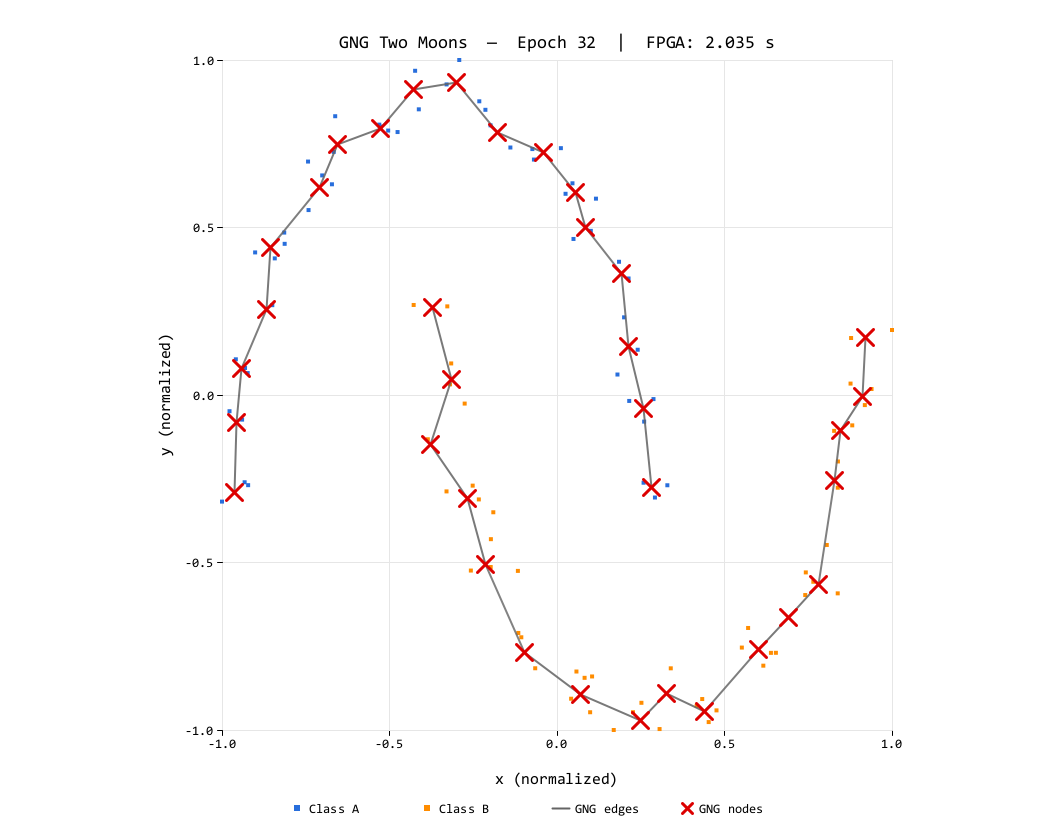
\includegraphics[width=0.48\textwidth]{two_moons_result.png}
\caption{Learned GNG topology on Two Moons (100 samples; $N_{\max}\!=\!40$). Node positions received via UART and plotted in normalized $[-1,1]$ coordinates.}
\label{fig:two_moons_result}
\end{figure}

\begin{figure}[!h]
\centering
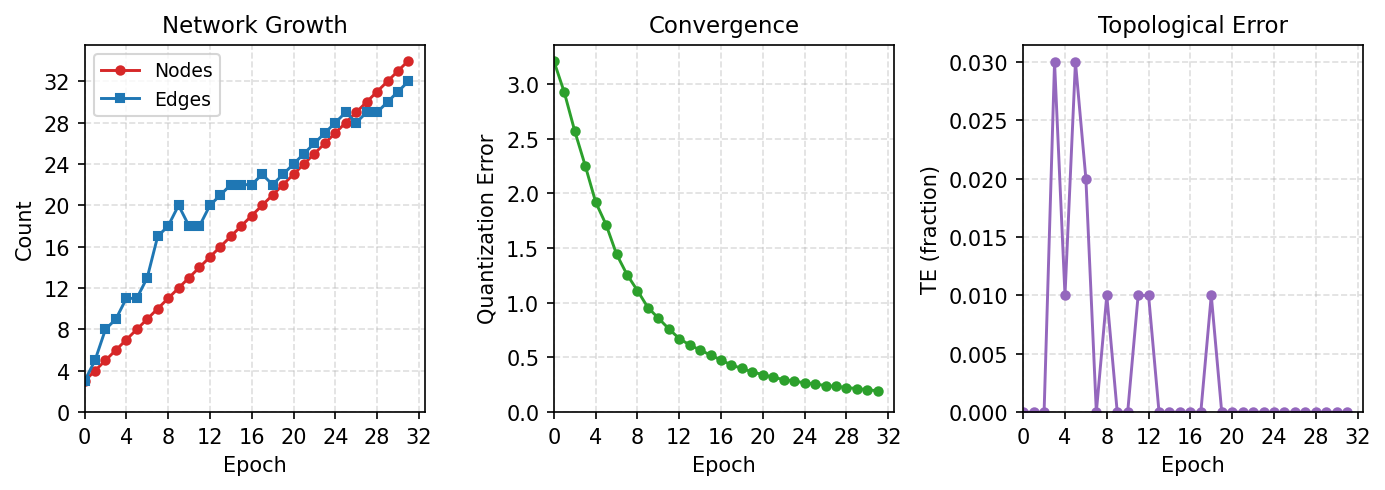
\includegraphics[width=0.48\textwidth]{two_moons_training.png}
\caption{Two Moons training dynamics over 32 epochs (100 samples/epoch). Left: node and edge count growth. Middle: quantization error convergence. Right: topological error vs. epoch.}
\label{fig:two_moons_training}
\end{figure}

\begin{figure}[t]
\centering
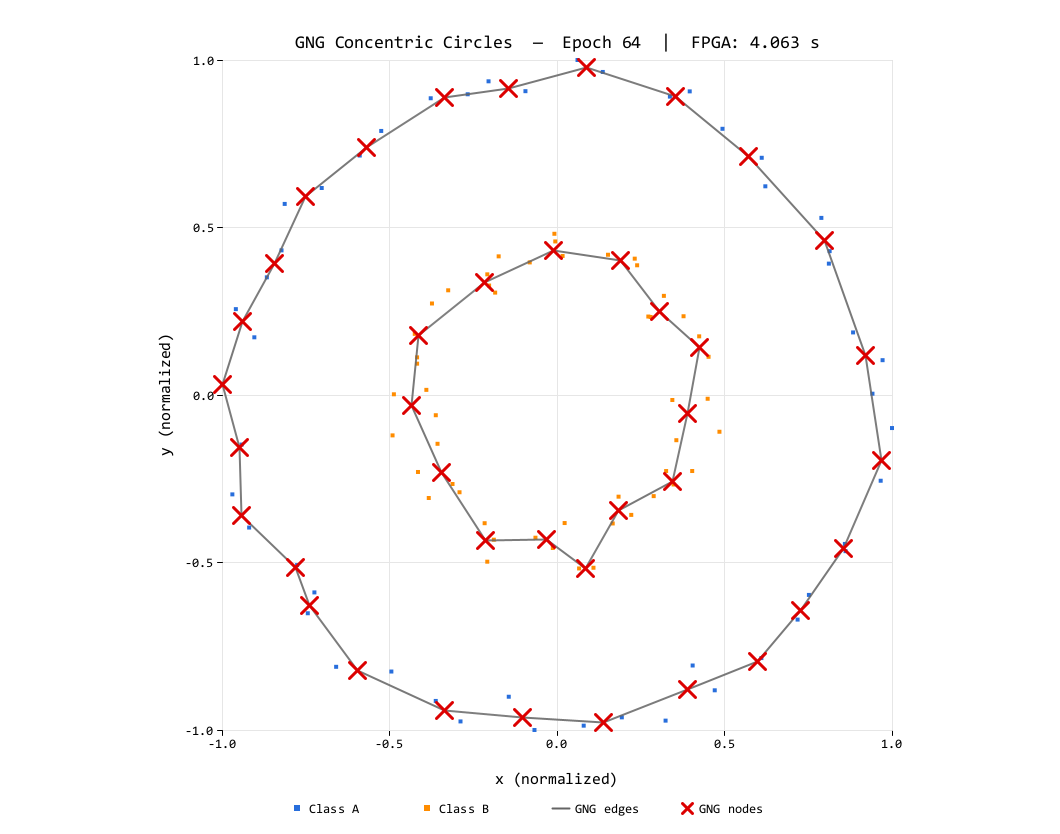
\includegraphics[width=0.48\textwidth]{concentric_circles_result.png}
\caption{Learned GNG topology on Concentric Circles (100 samples; $N_{\max}\!=\!40$).}
\label{fig:circles_result}
\end{figure}

\begin{figure}[t]
\centering
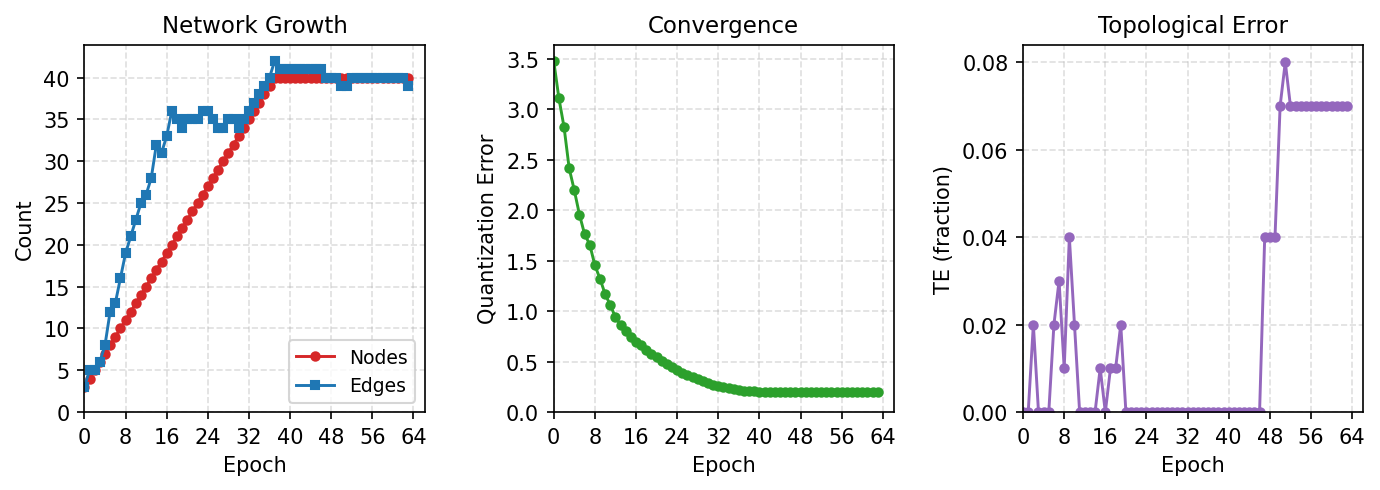
\includegraphics[width=0.48\textwidth]{concentric_circles_training.png}
\caption{Concentric Circles training dynamics over 64 epochs (100 samples/epoch). Left: network growth. Middle: quantization error convergence. Right: topological error vs. epoch.}
\label{fig:circles_training}
\end{figure}

\subsection{Computational Performance}
Table~\ref{tab:runtime} reports per-sample latency and throughput, measured directly from the 32-bit cycle counter embedded in each DBG frame (Section~\ref{sec:arch}) and converted using the 27~MHz clock. Per-sample latency is the cycle difference between consecutive frames; total training time is the span from the first to the last frame. Both datasets exhibit consistent latency of $\sim$625~$\mu$s ($\sim$16{,}900 cycles), yielding $\sim$1{,}600 samples/s. The latency is dominated by the WIN\_SCAN and NB\_SCAN passes, each requiring $N_{\max}$ sequential BRAM read-modify-write sequences, and is further gated by the per-sample UART debug transmission; the FSM computation alone completes in fewer cycles. This deterministic, bounded latency confirms that the design meets real-time constraints for sample-by-sample processing at moderate data rates.

\begin{table}[!h]
\centering
\caption{FPGA runtime performance
 at 27~MHz ($N_{\max}=40$).}
\label{tab:runtime}
\footnotesize
\setlength{\tabcolsep}{3pt}
\resizebox{\columnwidth}{!}{%
\begin{tabular}{l r r r r}
\toprule
\textbf{Dataset} & \textbf{Cycles/sample} & \textbf{$\mu$s/sample} & \textbf{Samples/s} & \textbf{Total (s)} \\
\midrule
Two Moons          & 16{,}852 & 624.1 & 1{,}602 & 5.40 \\
Concentric Circles & 16{,}931 & 627.1 & 1{,}595 & 5.72 \\
\bottomrule
\end{tabular}}
\end{table}

% ============================================================
\section{Discussion}

\subsection{Hardware Trade-offs}

\subsubsection{Sequential FSM vs. Parallel Datapath}
The sequential FSM minimizes LUT usage at the cost of $O(N_{\max})$ per-sample latency. A parallel winner-search tree could reduce this to $O(\log N_{\max})$ at the expense of additional LUTs.

\subsubsection{Integer Approximation of Learning Rates}
The Q8 and Q16 shift-scaled learning rates ($\epsilon_w \approx 0.301$, $\epsilon_n \approx 0.001$) are hardware-friendly but not exact. A winner rate of 0.3 rather than the canonical 0.05 causes faster convergence but may slightly increase quantization error. A finer Q8 approximation (e.g., \texttt{EPS\_WIN\_Q8}$=13$ for $\approx 0.05$) can be substituted without circuit changes. Despite these approximations, the final QE and TE reported in Table~\ref{tab:qe_te} remain low on both benchmarks, indicating that the shift-based rates are acceptable for the tested datasets.

\subsubsection{Isolated-Node Policy}
Canonical GNG deactivates a node when it loses all edges. Our FSM instead retains isolated nodes (\texttt{deg}$=0$) in BRAM and continues to include them in winner selection. This avoids cascaded deactivation logic and allows the node to re-acquire edges in subsequent iterations. The trade-off is that an isolated node occupies one of the $N_{\max}$ slots without contributing to topology coverage until it regains connectivity.

\subsubsection{Error Accumulation Scaling}
The \texttt{ERR\_SHIFT}$=4$ factor prevents 32-bit overflow; for larger coordinate ranges or longer training, this parameter should be increased.

\subsection{Relation to Prior FPGA Self-Organizing Work}
Prior FPGA SOM designs~\cite{coelho2020fpga,Dias2021SOMFPGA} assume static lattice connectivity. GNG requires per-iteration edge read-modify-write on a variable-structure graph, motivating the BRAM-indexed edge-cell representation. Our results show that full self-organizing clustering with dynamic topology is feasible on a sub-10K-LUT device.

\subsection{Relation to GNG Variants and Continual Learning}
This work follows the core update structure of canonical GNG~\cite{fritzke1994growing} while introducing hardware-oriented approximations to keep the design synthesizable and comparable. The algorithm inherently supports incremental adaptation through error-driven growth and age-based pruning, properties relevant to continual learning. Extensions such as GWR~\cite{marsland2002self}, utility-based management~\cite{Holmstrom2002Utility}, and drift-adaptive approaches~\cite{Arostegi2025AiGAS} could benefit from similar edge-cell and integer-arithmetic design.

\subsection{Limitations and Future Works}
The current evaluation uses two static 2D benchmarks; validation on non-stationary streaming data remains future work. The present results therefore demonstrate that the hardware substrate supports correct topology learning, but do not yet confirm adaptation under distribution shift.

Future work targets four directions: (i) \emph{continual learning on FPGA}---extending the design to accept streaming sensor data and adapt continuously without restarting; (ii) \emph{parallel winner search}---replacing the sequential scan with a pipelined tree to reduce latency to $O(\log N_{\max})$; (iii) \emph{configurable precision}---parameterizing Q-format constants via generics; and (iv) \emph{multi-stream input}---accepting real-time sensor data for on-board unsupervised mapping.


% ============================================================
\section{Conclusion}
This paper presented an FPGA implementation of GNG on the Sipeed Tang Nano 9K (Gowin GW1NR-9C) as a bounded-memory substrate for online self-organizing clustering. The edge-cell graph encoding halves edge-storage relative to a dense adjacency baseline, and a fused NB\_SCAN pass combines error decay, edge aging, and neighbor adaptation into a single sweep. On Two Moons and Concentric Circles, the integer-only datapath preserves good topology learning quality with deterministic per-sample latency, showing that Q8/Q16 fixed-point arithmetic and shift-based learning rates are sufficient on the evaluated datasets. These results demonstrate that self-organizing clustering can be deployed on sub-10K-LUT FPGAs when memory layout and arithmetic format are treated as first-class design concerns. Because GNG processes samples incrementally with bounded state, the proposed platform provides a hardware foundation for continual learning on resource-constrained edge devices.

\section*{Acknowledgment}
This work was supported by the Japan Science and Technology Agency (JST), Moonshot R\&D Program, under grant number JPMJMS2034.

The authors used Anthropic Claude Opus 4.6 to refine wording and clarity. All technical content and results were verified by the authors, who take full responsibility for the paper.
\bibliographystyle{IEEEtran}
\bibliography{references}

\end{document}
